\chapter{ระบบต้นแบบ}
\label{chapter:result}

\section{การออกแบบส่วนต่อประสานกับผู้ใช้งาน}

ส่วนต่อประสานกับผู้ใช้งาน และหน้าที่การทำงานของแต่ละส่วนของระบบทั้งส่วนแสดงสถิติการทดสอบและส่วนการจัดการรายชื่อของผู้สมัครทดสอบ มีรายละเอียดดังนี้

\subsection{หน้าแสดงสถิติและประเภทการทดสอบ}

การแสดงสถิติกรณีผู้ใช้คือผู้ดูแลระบบ (Admin) ผู้ใช้สามารถเห็นหน้าจอดังกล่าวซึ่งจะแสดงคะแนนต่าง ๆ ของการทดสอบครั้งก่อนและการทดสอบในครั้งปัจจุบัน และสามารถเห็นปุ่มต่าง ๆ ที่สามารถจัดการประเภทการทดสอบได้ ดังแสดงในรูปที่ \ref{fig:admin-contest-dashboard}

\begin{figure}[H]
    \centering
    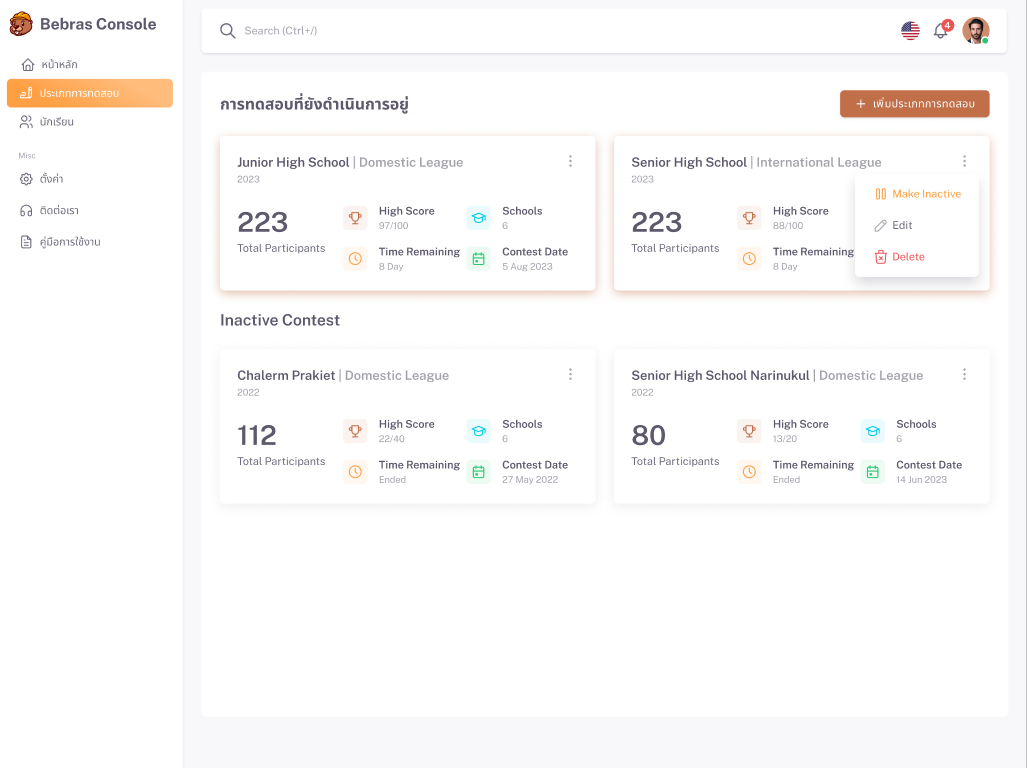
\includegraphics[width=100mm,scale=1.0]{images/editCon.png}
    \caption{หน้าแสดงสถิติและประเภทการทดสอบสำหรับผู้ดูแลระบบ}
    \label{fig:admin-contest-dashboard}
\end{figure}

การแสดงสถิติกรณีผู้ใช้คือผู้ประสานงาน (Coordinator) ผู้ใช้สามารถเห็นหน้าจอดังกล่าวซึ่งจะแสดงคะแนนต่าง ๆ ของการทดสอบครั้งก่อนและการทดสอบในครั้งปัจจุบัน ดังแสดงในรูปที่ \ref{fig:teacher-contest-dashboard}

\begin{figure}[H]
    \centering
    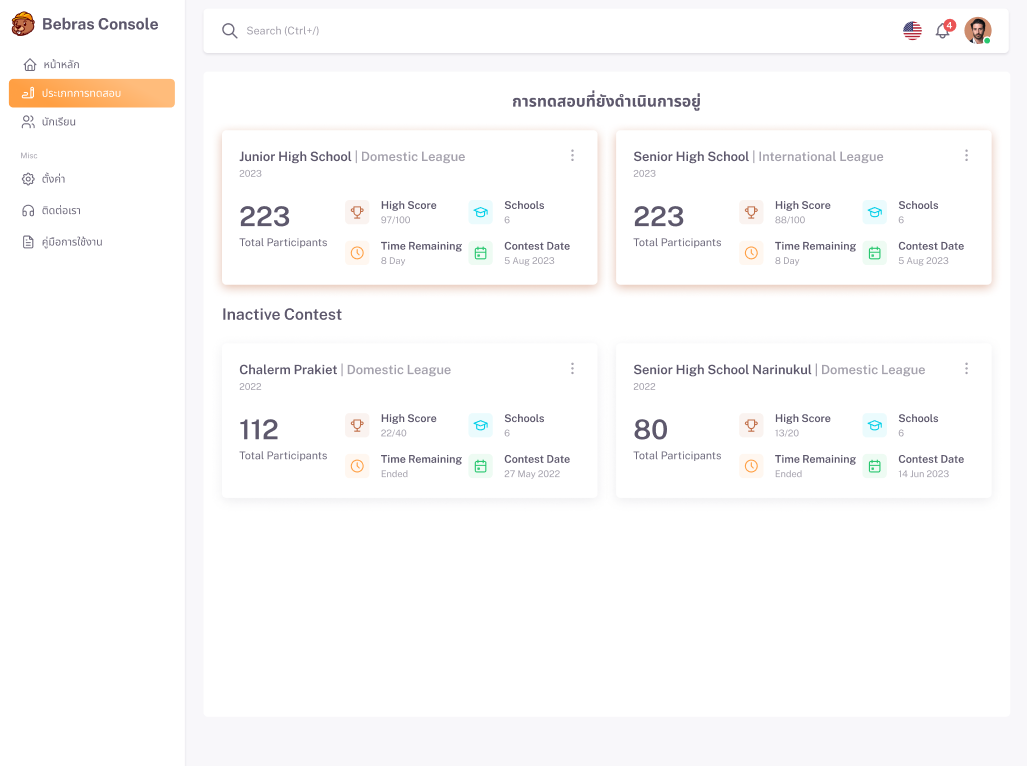
\includegraphics[width=100mm,scale=1.0]{images/statisTeacher.png}
    \caption{หน้าแสดงสถิติและประเภทการทดสอบสำหรับผู้ประสานงาน}
    \label{fig:teacher-contest-dashboard}
\end{figure}

\subsection{หน้าแสดงสถิติของนักเรียนในแต่ละการทดสอบ}

การแสดงสถิติกรณีผู้ใช้คือผู้ประสานงาน (Coordinator) ผู้ใช้สามารถเห็นผลคะแนนการเข้าทดสอบของนักเรียนแต่ละคนได้ ดังแสดงในรูปที่ \ref{fig:admin-contest-stats}

\begin{figure}[H]
    \centering
    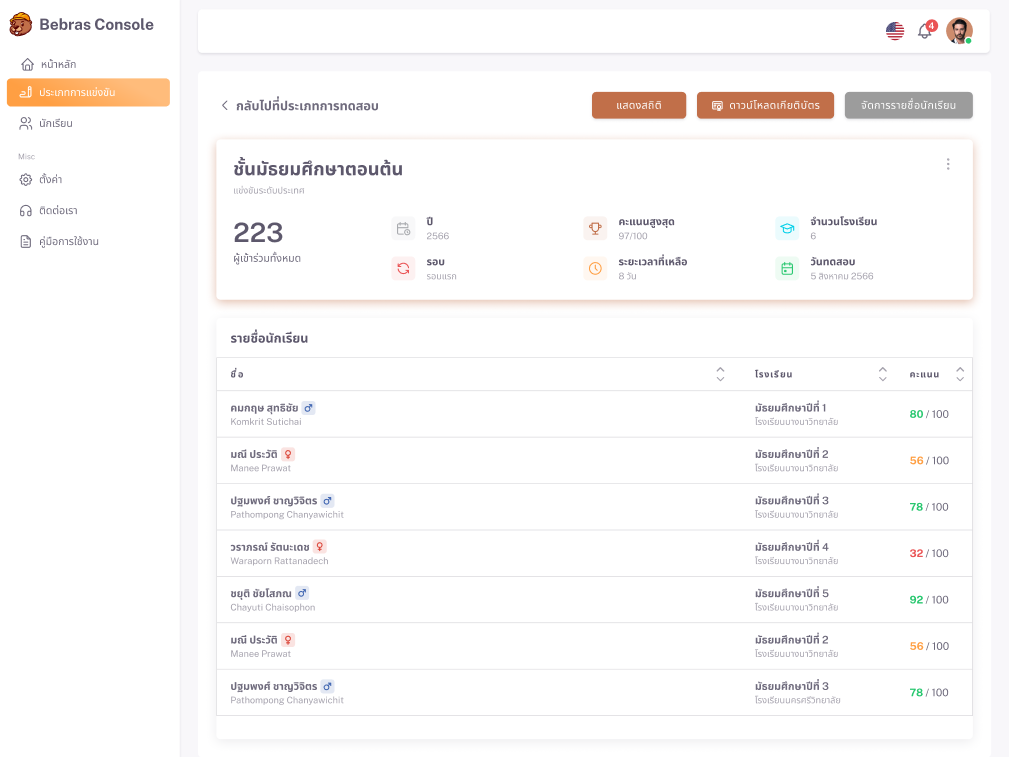
\includegraphics[width=100mm,scale=1.0]{images/teacherScore.png}
    \caption{หน้าแสดงสถิติของนักเรียนในแต่ละการทดสอบสำหรับผู้ประสานงาน}
    \label{fig:admin-contest-stats}
\end{figure}

การแสดงสถิติกรณีผู้ใช้คือผู้ประสานงาน (Coordinator) ผู้ใช้สามารถเห็นสถิติคะแนนและข้อมูลการทดสอบต่าง ๆ ของนักเรียนแต่ละคนได้ ทั้งยังสามารถกดดาวน์โหลดข้อมูลของสถิตินั้น ๆ ได้ ดังแสดงในรูปที่ \ref{fig:teacher-contest-stats}

\begin{figure}[H]
    \centering
    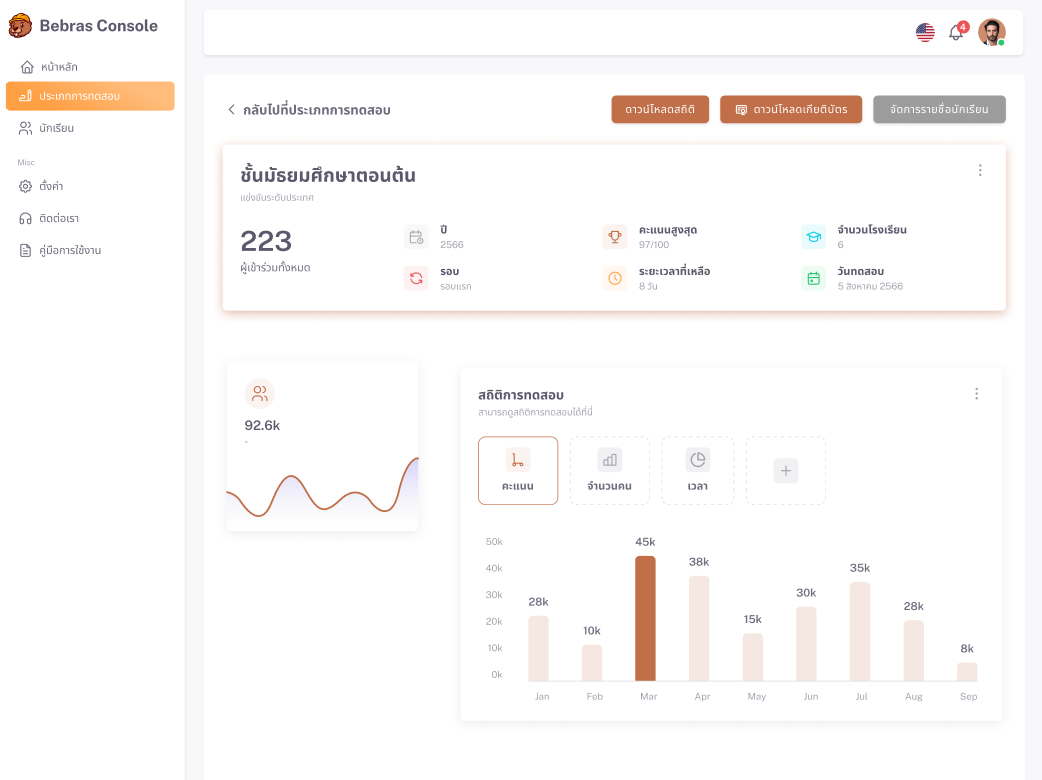
\includegraphics[width=100mm,scale=1.0]{images/statistic.png}
    \caption{หน้าแสดงสถิติของนักเรียนในแต่ละการทดสอบสำหรับผู้ประสานงาน}
    \label{fig:teacher-contest-stats}
\end{figure}

\subsection{หน้าแสดงรายชื่อนักเรียน}

เมื่อเข้าสู่หน้า Student ระบบจะแสดงรายชื่อนักเรียนทั้งหมดที่มีอยู่ในระบบ โดยสามารถเพิ่มข้อมูลของนักเรียน (Student) ได้ในหน้านี้โดยการคลิกที่คำว่า "เพิ่มรายชื่อนักเรียน" เพื่อเพิ่มข้อมูลของนักเรียนลงในระบบได้ ดังรูปที่ \ref{fig:dashboard-student}

\begin{figure}[H]
    \centering
    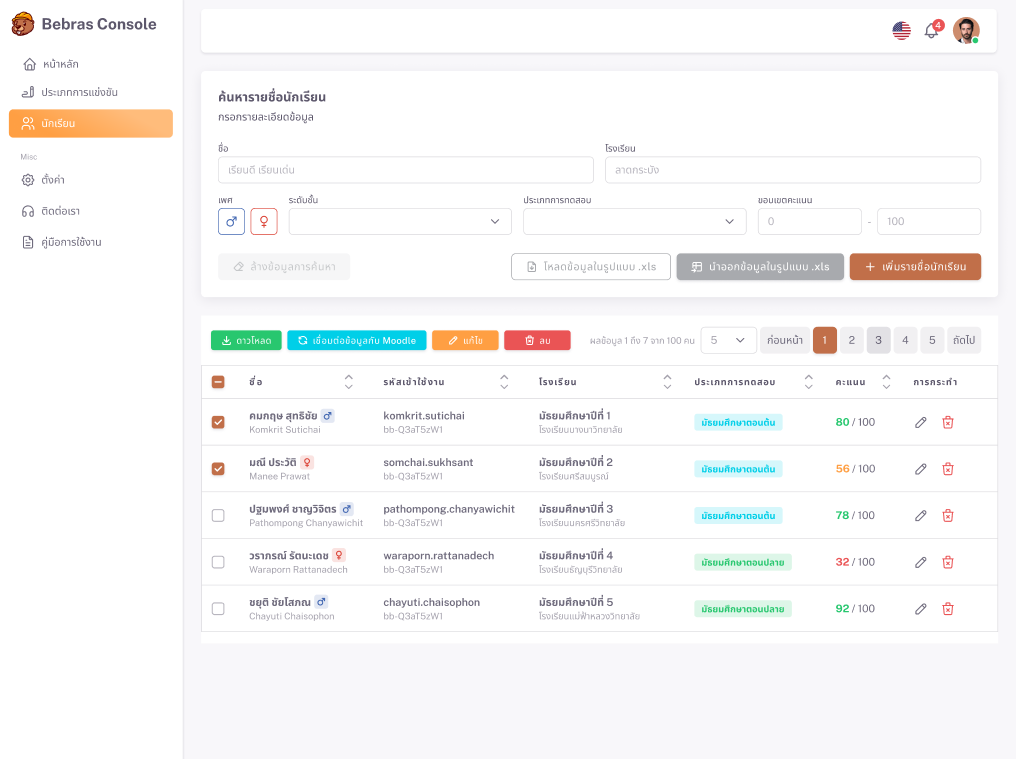
\includegraphics[width=100mm,scale=1.0]{images/students.png}
    \caption{หน้าแสดงรายชื่อนักเรียน}
    \label{fig:dashboard-student}
\end{figure}

\subsection{หน้าเพิ่มรายชื่อนักเรียน}

โดยหลังจากคลิกที่ปุ่ม "เพิ่มรายชื่อนักเรียน" ระบบจะแสดงหน้าต่างให้กรอกข้อมูลของนักเรียน ดังแสดงในรูปที่ \ref{fig:addStudent}

\begin{figure}[H]
    \centering
    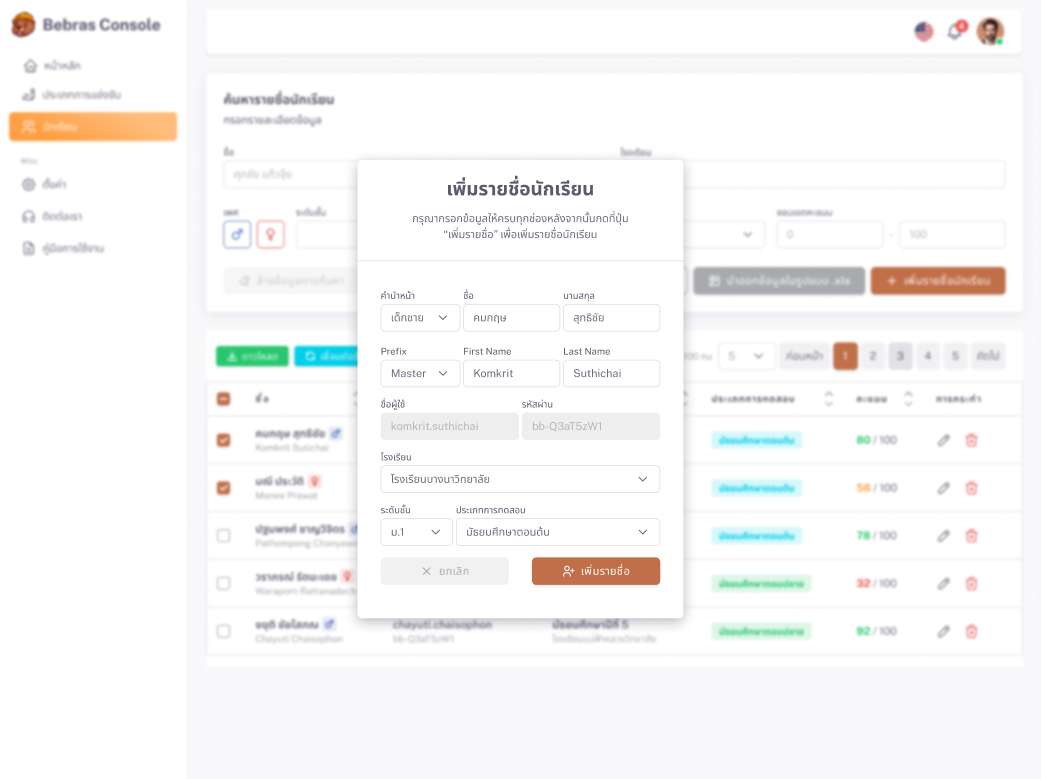
\includegraphics[width=100mm,scale=1.0]{images/addStudent.png}
    \caption{หน้าเพิ่มรายชื่อนักเรียน}
    \label{fig:addStudent}
\end{figure}

\subsection{หน้าลบรายชื่อนักเรียน}

ผู้ดูแลระบบ (Admin) หรือผู้ประสานงาน (Coordinator) สามารถลบข้อมูลของนักเรียน (Student) ได้ในหน้านี้โดยการคลิกที่ปุ่มถังขยะในแถวของนักเรียนที่ต้องการลบ ดังแสดงในรูปที่ \ref{fig:dashboard-student} หลังจากนั้นจะมีพอปอัพเพื่อให้ผู้ใช้ยืนยันก่อนทำการลบ ดังแสดงในรูปที่ \ref{fig:remove-student}

\begin{figure}[H]
    \centering
    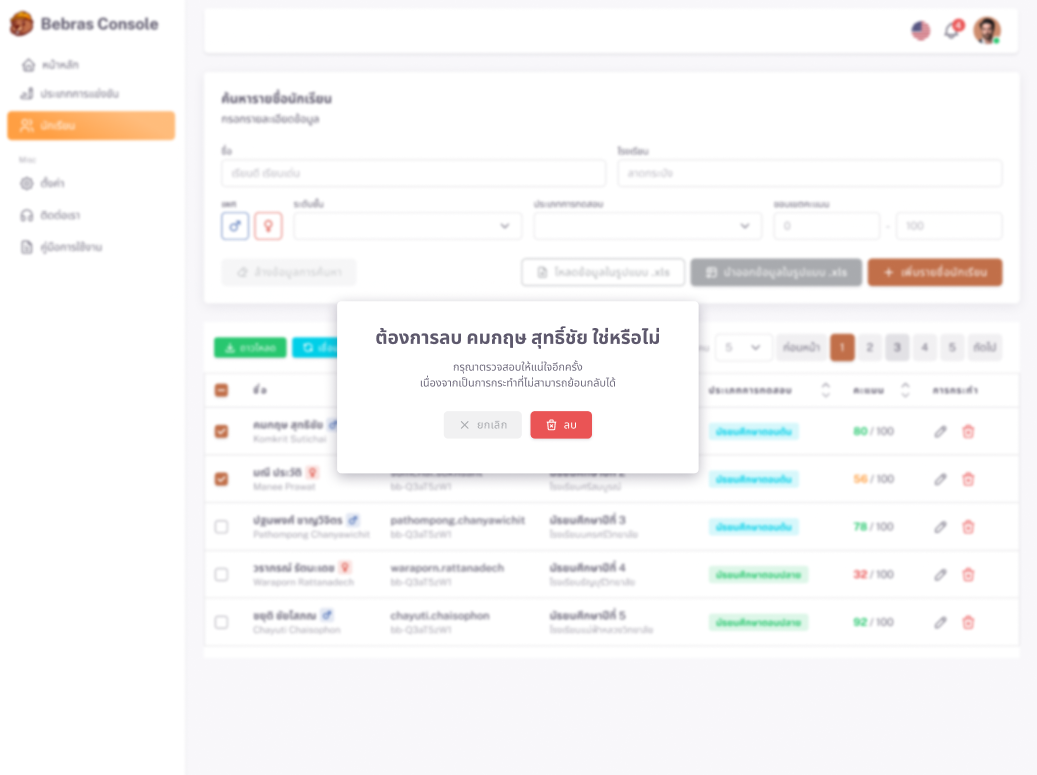
\includegraphics[width=100mm,scale=1.0]{images/deleteStudent.png}
    \caption{หน้าลบรายชื่อนักเรียน}
    \label{fig:remove-student}
\end{figure}

\subsection{หน้าเพิ่มนักเรียนเป็นกลุ่ม}

ผู้ดูแลระบบ (Admin) หรือผู้ประสานงาน (Coordinator) สามารถเพิ่มข้อมูลของนักเรียน (Student) ได้ในหน้านี้โดยการคลิกที่ปุ่ม "นำเข้ารูปรายชื่อนักเรียนในรูปแบบ .xlsx" ดังแสดงในรูปที่ \ref{fig:dashboard-student} เมื่อทำการคลิกปุ่มดังกล่าวจะปรากฎพอปอัพดังรูปที่ \ref{fig:addStudentGroup}

\begin{figure}[H]
    \centering
    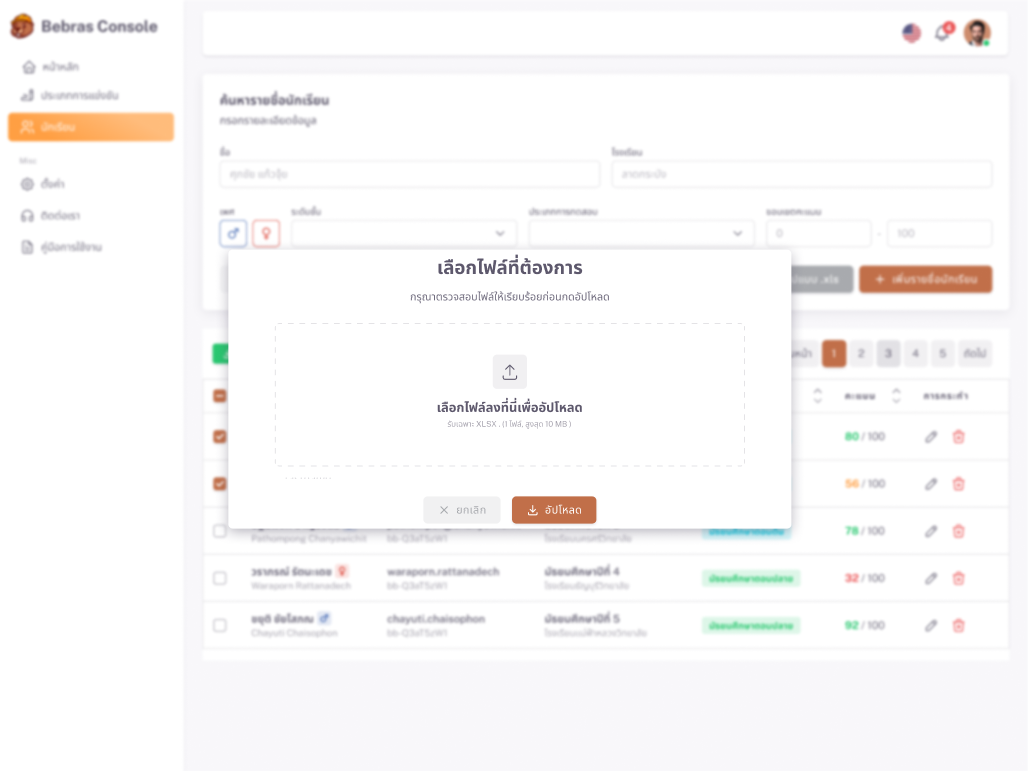
\includegraphics[width=100mm,scale=1.0]{images/addStudentGroup.png}
    \caption{การเพิ่มนักเรียนเป็นกลุ่ม}
    \label{fig:addStudentGroup}
\end{figure}

\subsection{หน้าการแก้ไขข้อมูลนักเรียน}

ผู้ดูแลระบบ (Admin) หรือผู้ประสานงาน (Coordinator) สามารถแก้ไขมูลของนักเรียน (Student) ได้ในหน้านี้โดยการคลิกที่ไอคอนรูปปากกา ดังแสดงในรูปที่ \ref{fig:dashboard-student} เมื่อทำการคลิกไอคอนดังกล่าวจะปรากฎพอปอัพดังรูปที่ \ref{fig:editStudent}

\begin{figure}[H]
    \centering
    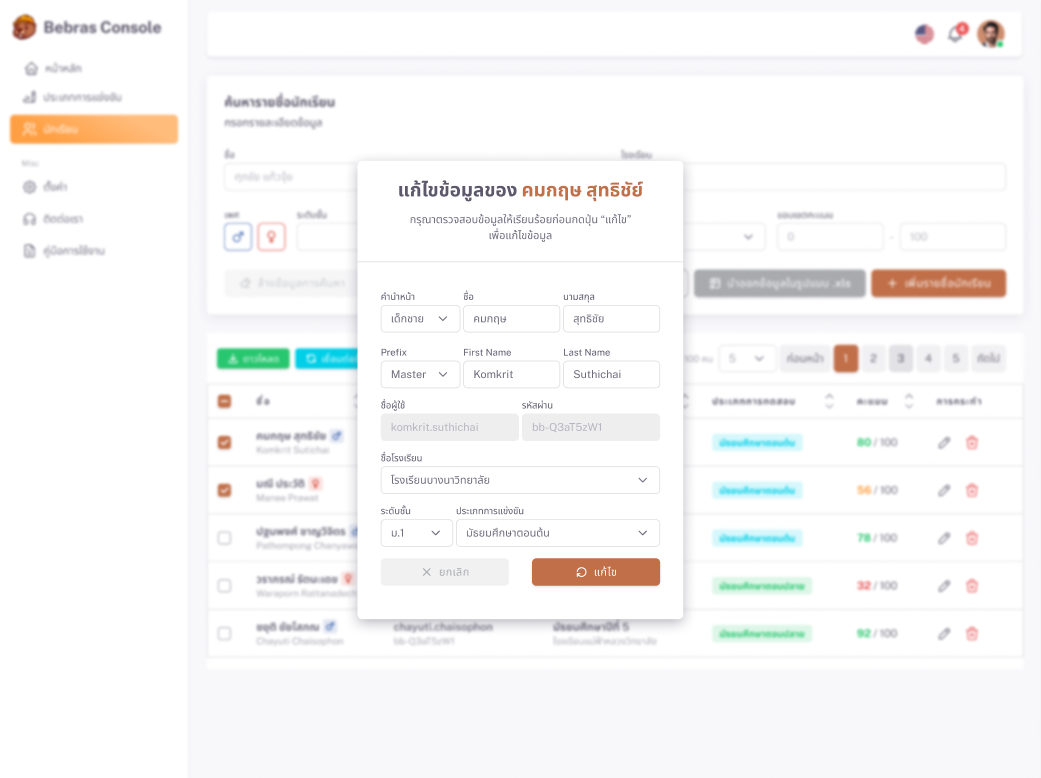
\includegraphics[width=100mm,scale=1.0]{images/editStudent.png}
    \caption{การแก้ไขข้อมูลนักเรียน}
    \label{fig:editStudent}
\end{figure}


